\chapter{Desenvolvimento do trabalho}\label{cap:desenvolvimento_trabalho}
Essa seção apresenta o que foi realizado no trabalho.

Como exposto em \cite{Torralba2008}, o aprendizado de máquina tem sido utilizado como alternativa à implementação de algoritmos\index{algoritmo} específicos e complexos durante a resolução de diversos tipos de problemas. 

\lipsum[6]

A Figura \ref{fig:mlapplications}, apresenta um breve resumo das possíveis aplicações do aprendizado de máquina.

\begin{figure}[ht]
    \centering
    \caption{Domínio de aplicações do aprendizado de máquina.}
    \copyrightbox[b]
    		{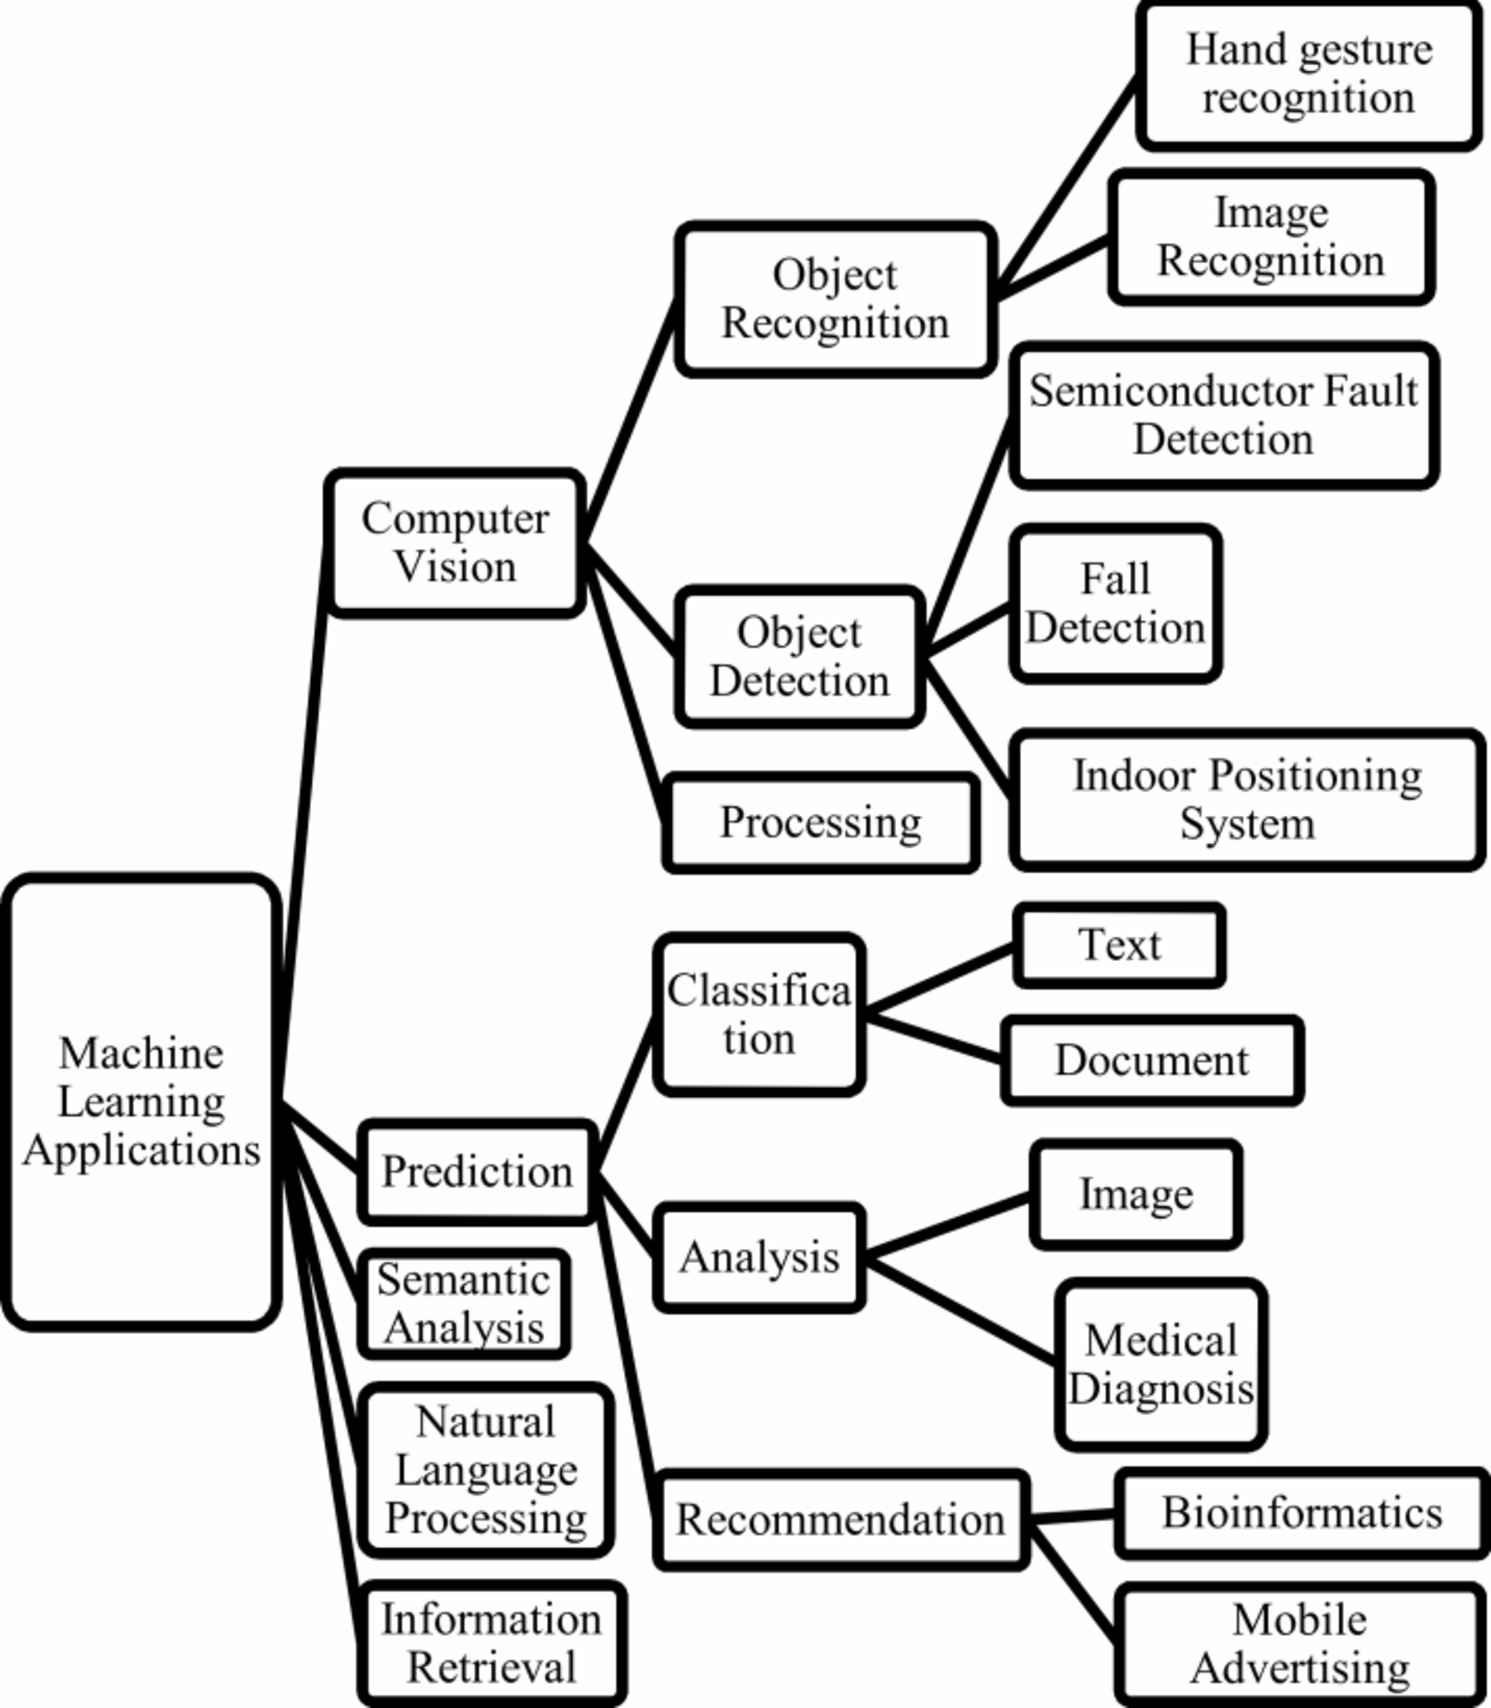
\includegraphics[width=0.7\linewidth]{mlapplications}}
            {Fonte: Extraída de \cite{ApplicationMachineLearning}}
    \label{fig:mlapplications}
\end{figure}

\lipsum[22]

\section{Assunto 1 do desenvolvimento do trabalho}

Como apresentado em \cite{mohri2018foundations}, com o resultado do desenvolvimento das tecnologias web, das redes sociais\index{redes sociais} e dispositivos móveis\index{dispositivos móveis}, ocorreu uma verdadeira explosão no crescimento dos dados\index{dados}. 

\lipsum[23-27]

\section{Assunto 2 do desenvolvimento do trabalho}

\lipsum[23-27]

\begin{enumerate}
    \item Exemplo de litstagem enumerada de algoritmo\index{algoritmo};
    \item Outro exemplo de de litstagem enumerada;
    \item Último exemplo de listagem enumerada.
\end{enumerate}

\lipsum[28]:

\begin{itemize}
    \item Exemplo de listagem com bullets;
    \item Outro exemplo de listagem com bullets; 
    \item Exemplo final de listagem com bullets. 
\end{itemize}
